\section{Results}

\subsection{\label{sec:gridstudy}Domain and grid resolution study}

In order to ensure that the large and small turbulence scales were
properly resolved in the offshore LES simulations, the appropriate
domain size and mesh resolution needed to be determined.
Under-resolved meshes or domain sizes which are too small may miss the
smaller turbulence scales or remove the larger structures required for
proper ABL development.  However, over-resolved meshes or
unnecessarily large domains might lead to excessive computational
requirements to complete the simulations.

To determine the appropriate mesh size and resolution, a grid study
was conducted using the stable 5m/s ABL case and the Nalu-Wind code.
A number of cases were set up using the surface roughness and
prescribed temperature decreases listed in table
\ref{tab:z0tempparam}, but with varying grid resolutions and
conservative estimates for the domain size required.  As shown in
table \ref{tab:GridStudySetup}, the horizontal resolutions varied from
10m to 2.5m cells for the coarse and fine cases, respectively.  All
simulations for the grid study also used a vertical resolution of
dz=2.5m and the same vertical extent of 1km.

%%%%%%%%%%%%%%% GRID STUDY: INTEGRAL LENGTH %%%%%%%%%%%%%%%%%%%%%%%%
\begin{table}
\caption{\label{tab:GridStudySetup} The setup for the grid resolution study} \centering
\begin{tabular}{ccccc}
  \hline
  Case              & dx [m] & dy [m] & dz [m] & Domain size \\
  \hline
  Nalu-wind coarse  &  10.0  & 10.0   & 2.5 & 1.5km $\times$ 1.5km $\times$ 1.0km  \\
  Nalu-wind medium  &   5.0  &  5.0   & 2.5 & 1.5km $\times$ 1.5km $\times$ 1.0km  \\
  Nalu-wind fine    &   2.5  &  2.5   & 2.5 & 1.0km $\times$ 1.0km $\times$ 1.0km  \\
% AMR-wind fine     &   2.5  &  2.5   & 2.5 & 0.0 \\
\hline
\end{tabular}
\end{table}
%%%%%%%%%%%%%%%%%%%%%%%%%%%%%%%%%%%%%%%%%%%%%%%%%%%%%%%%%%%%%%%%%%%%

The suitability of these meshes and domain sizes were determined based
on the resulting wind spectra and turbulent correlation metrics from
the simulated ABL. The wind spectra $S_i(f)$ is defined as a function
of the frequency $f$
\begin{equation}
  \int_0^\infty S_i(f) \textrm{d}f = \sigma_i^2
\end{equation}
where $\sigma_i$ is the wind speed variance and the index $i=u,v,w$
denotes the longitudinal, lateral, or vertical velocity, respectively.
For the LES simulations in this study, we desire that that the mesh
resolution be sufficiently fine to capture the high frequency
components of the spectra past the spectral peak.  This helps ensure
that the unsteady characteristics in the boundary layer are resolved.


%%%%%%%%%%% Grid resolution spectra figure %%%%%%%%%%%%%%%%%%%%%%%%%
% Created in Postprocessing/GridStudy/GridStudy_Spectra.ipynb
\begin{figure}%[hbt!]
  \centering
  \fxnote{remove AMR-Wind results from graphs}\\
  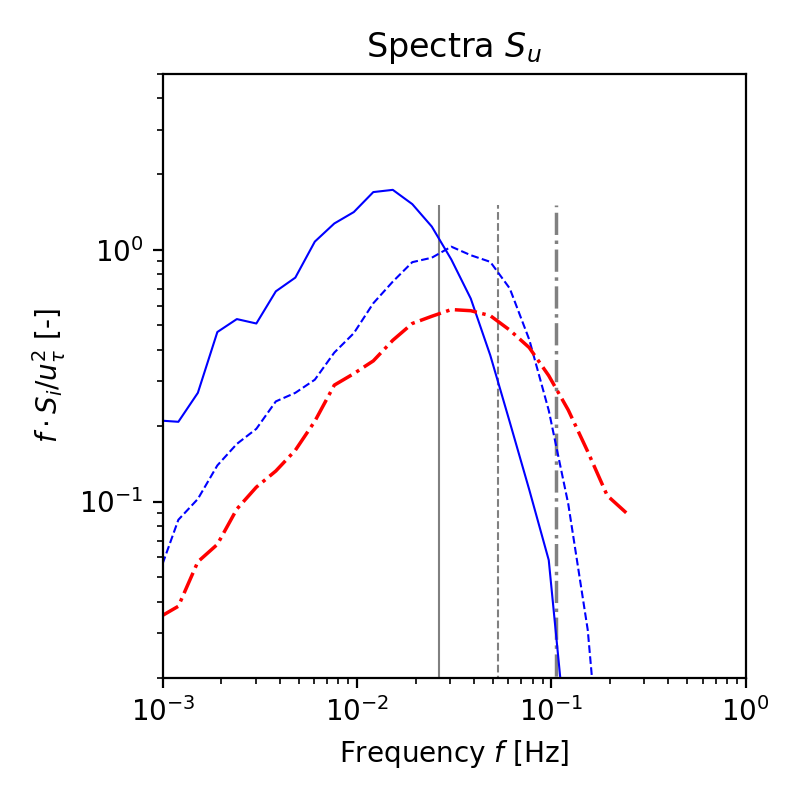
\includegraphics[width=2.0in]{figures/GridStudy_Spectra_Su.png}
  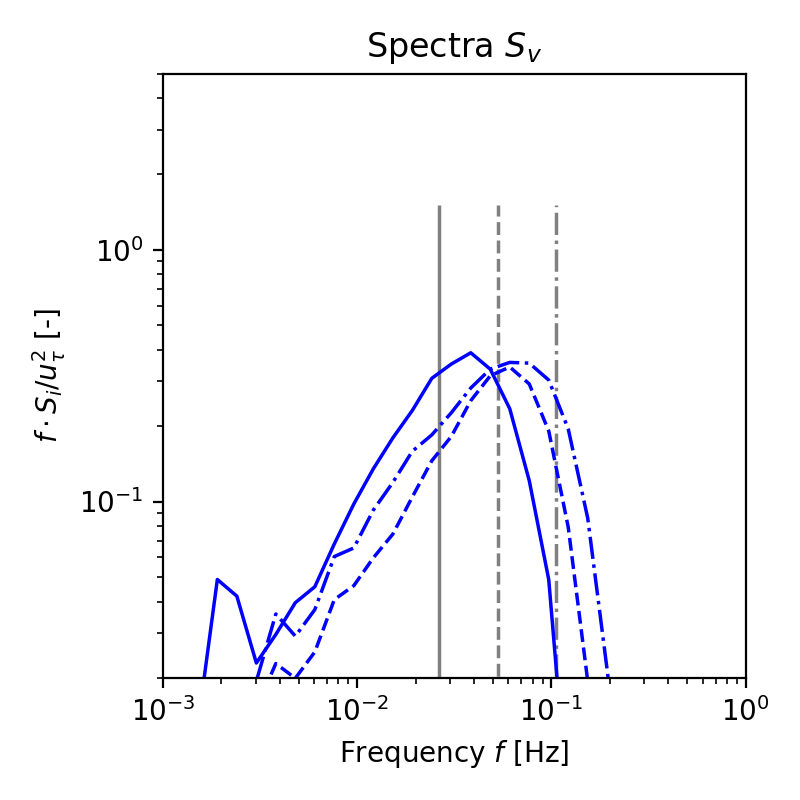
\includegraphics[width=2.0in]{figures/GridStudy_Spectra_Sv.png}
  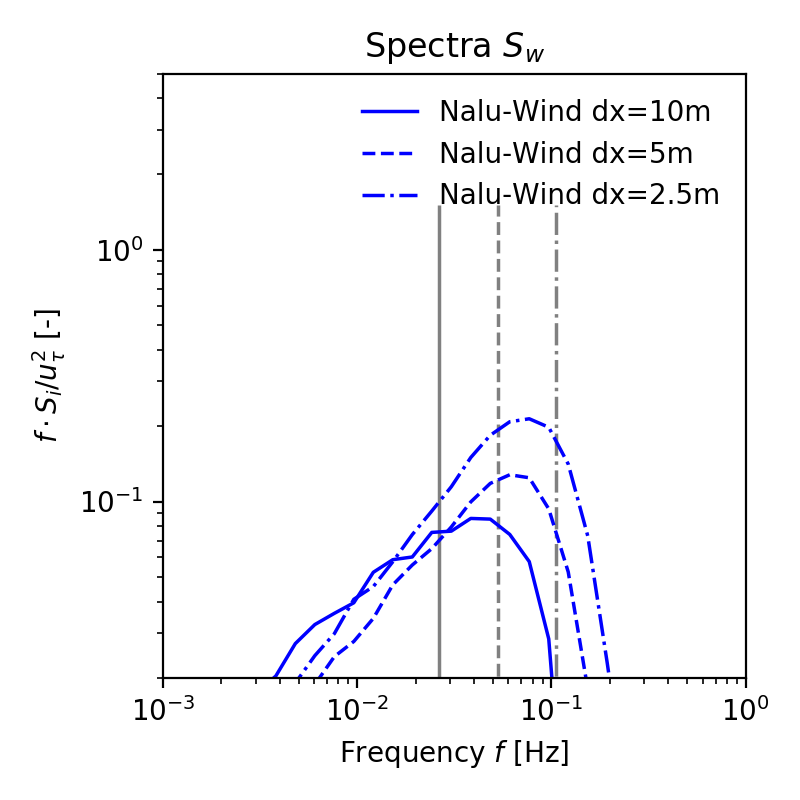
\includegraphics[width=2.0in]{figures/GridStudy_Spectra_Sw.png}
  \caption{   \label{fig:GridStudySpectra} 
    Calculation of the wind spectra $S_i$ for LES of stable
    5m/s case with different resolutions.  The gray vertical lines
    correspond to the maximum resolvable frequency $f_{max}$ according
    to equation (\ref{eq:fmax}). }
\end{figure}
%%%%%%%%%%%%%%%%%%%%%%%%%%%%%%%%%%%%%%%%%%%%%%%%%%%%%%%%%%%%%%%%%%%%

Two numerical constraints limit the maximum resolvable frequency in
the current ABL computations.  First, the Nyquist frequency $f_{Ny}$
limits the highest resolved frequency to half the sampling frequency, or

\begin{equation}
  f_{Ny} = \frac{1}{2\times \textrm{dt}}
\end{equation}
Secondly, the maximum resolvable frequency of convecting fine scale
eddies on a mesh with grid size $\Delta$ and average horizontal wind
speed $\bar{U}_{horiz}$ can be estimated as
\begin{equation}
  \label{eq:fmax}
  f_{max} = \frac{0.6\bar{U}_{horiz}}{N\Delta}.
\end{equation}
Here, equation \ref{eq:fmax} assumes that the turbulent eddies convect
with a velocity of $0.6\bar{U}_{horiz}$ and $N=8$ is chosen for the
purposes of this study.  Due to the alignment of the flow with the
mesh directions, the grid size $\Delta = \sqrt{2}\cdot \textrm{dx}$.
In all cases considered here, $f_{max} < f_{Ny}$, so the limiting
constraint for resolving the high frequency components was the mesh
resolution.

The comparison of the wind spectra and maximum resolvable frequency
$f_{max}$ for the different mesh resolutions is shown in figure
\ref{fig:GridStudySpectra}.  Here spectra is shown at the $z$=20m
height and averaged using 1/3 octave-bins to enchance clarity. For the
$S_u$ and $S_w$ spectra, there noticeable shifts in the peak
amplitude, while the peak amplitudes for $S_v$ remained fairly
constant between cases.  In all cases, the peak frequency of $S_i(f)$
also increased as the resolution increased. While the mesh resolution
was sufficient to capture the peak frequency for $S_u$, the fine
resolution with 2.5m mesh cells was required to capture the spectral
peaks in the lateral and vertical directions.

The second metric for determining the appropriate grid size and mesh
resolution is through the correlation tensor and turbulence integral
length scale.  The two-point correlation tensor
$R_{ij}(\mathbf{x},\boldsymbol{\xi})$ at position $\mathbf{x}$ and
separation vector $\boldsymbol{\xi}$ is defined as
\begin{equation}
  \label{eq:Rij}
  R_{ij}({\mathbf x},\boldsymbol{\xi}) = 
  \frac{\overline{ {u'_i(\mathbf{x}, t) u'_j(\mathbf{x}+\boldsymbol{\xi},t)} }}
       { \sqrt{\overline{ u'^2_i }} \sqrt{\overline{ u'^2_j}} }
\end{equation}
where the velocity fluctuations $u'_i$ are defined as 
\begin{equation}
  u'_i(\mathbf{x},t) = u_i(\mathbf{x},t) - \overline{ u_i(\mathbf{x},t) }
\end{equation}
and the overbar operator $\overline{(\bullet)}$ denotes time
averaging.  In the current study, we compute the horizontally averaged
correlation coefficient $\langle R_{ij}(\boldsymbol{\xi})\rangle$ by
sampling over multiple points at the $z$=20m height, typically 100-150
points, and averaging the result.  The longitudinal $\langle
R_{ij}(\boldsymbol{\xi})\rangle$ was calculated by looking at
separation vectors $\boldsymbol{\xi}$ in the streamwise direction
while the lateral $\langle R_{ij}(\boldsymbol{\xi})\rangle$ used
separation distances $\boldsymbol{\xi}$ which were orthogonal to the
wind direction on the same horizontal plane.

%%%%%%%%%%% Grid resolution Rij correlation figure %%%%%%%%%%%%%%%%%%%%
% Created in Postprocessing/GridStudy/GridStudy_Rij.ipynb
\begin{figure}%[hbt!]
  \centering
  \fxnote{remove AMR-Wind results from graphs}\\
  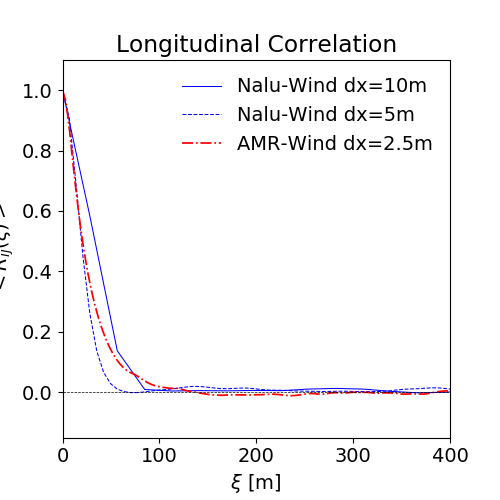
\includegraphics[width=2.5in]{figures/GridStudy_Rij_Longitudinal.png}
  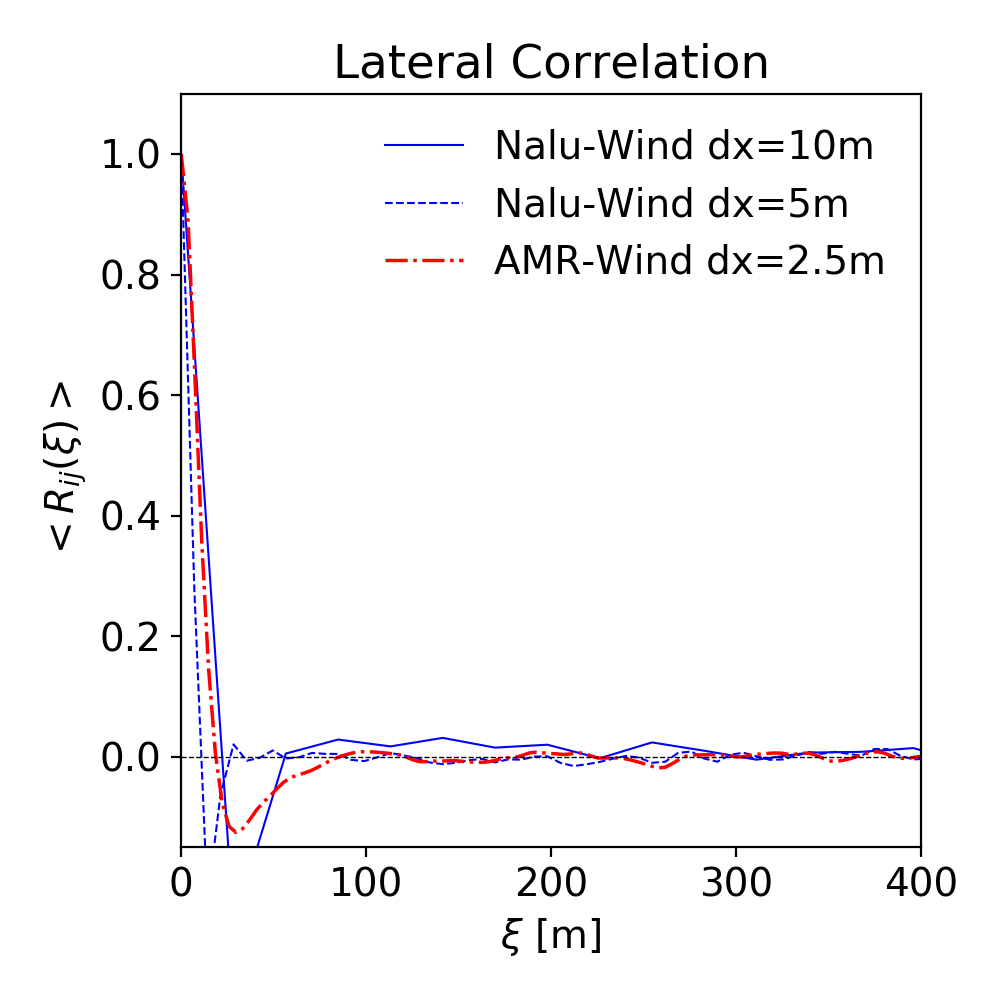
\includegraphics[width=2.5in]{figures/GridStudy_Rij_Lateral.png}
  \caption{\label{fig:GridStudyRij} Calculation of the averaged
    longitudinal and lateral $\langle R_{ij}(\boldsymbol{\xi})
    \rangle$ coefficient at $z$=20m for LES of stable 5m/s case with
    different resolutions.}
\end{figure}
%%%%%%%%%%%%%%%%%%%%%%%%%%%%%%%%%%%%%%%%%%%%%%%%%%%%%%%%%%%%%%%%%%%%

The results shown in figure \ref{fig:GridStudyRij} show that the
finest resolution is required to resolve both the longitudinal and the
lateral length scale.  In contrast to the neutral and unstable ABL
cases, the turbulent structures decorrelate rapidly and are noticeably
finer in the lateral direction compared to the longitudinal direction.
While 2.5m resolution is adequate to resolve the longitudinal
turbulent structures, the lateral direction may require even finer
resolution to fully resolve.  This may be an important consideration
in situations where turbulence in a stable boundary layer interacts
with turbine features, such as blade motions or downstream wakes.
However, the additional refinement requires careful balancing against
the additional computational expense in the simulation.

Similar conclusions can be drawn by examining the turbulent integral
length scale $L$.  This lengthscale can be calculated from $\langle
R_{ij}(\boldsymbol{\xi}) \rangle$ via
\begin{equation}
  L = \int_0^\infty \langle R_{ij}(\xi) \rangle \: {\textrm d}\xi
\end{equation}
and the results are shown in table \ref{tab:GridStudyLscale}.  With a
resolution of 2.5m, the ratio of the longitudinal length scale to the
grid size $L/\textrm{d}x \approx 10.1$, while in the lateral direction
$L/\textrm{d}x \approx 2.36$, suggesting even finer resolution is
required to capture the lateral scales.  Based on this longitudinal
length scale, we also determined the overall domain size necessary for
stable ABL calculations.  A minimum domain of 750m $\times$ 750m in
the horizontal directions was used in all Nalu-Wind and AMR-Wind LES
calculations, which provided sufficient space for the largest
turbulent structures to develop and evolve without interference from
the boundaries or other structures.

%%%%%%%%%%%%%%% GRID STUDY: INTEGRAL LENGTH %%%%%%%%%%%%%%%%%%%%%%%%%%%%%%%%%%%
\begin{table}[h!]
\caption{\label{tab:GridStudyLscale} The calculated turbulent integral
  lengthscale for each of the grid resolutions} \centering
\begin{tabular}{ccccc}
  \hline
  Case              & dx [m] & Longitudinal L  & Lateral L \\
  \hline
  Nalu-wind coarse  &  10.0  & 36.43 m         & 0.0 m     \\
  Nalu-wind medium  &   5.0  & 21.49 m         & 4.52 m    \\
  Nalu-wind fine    &   2.5  & 25.25 m         & 5.92 m    \\
% AMR-wind fine     &   2.5  & 27.689340 m     & 9.332672   \\
\hline
\end{tabular}
\end{table}

\subsection{Comparison of AMR-Wind vs Nalu-Wind}

%%%%%%%%%%%%%%% Compare Nalu/AMR integrated quantities %%%%%%%%%%%%%%
\begin{table}
\caption{\label{tab:CompareAMRvsNalu} Comparison of AMR-Wind and Nalu-Wind} \centering
\begin{tabular}{cccccc}
  \hline
  Code & Wind speed & TI      &  $\alpha$  &   $u_\tau$ \\ %&       L \\
  \hline
  Nalu-Wind & 5 m/s &  0.0481 &  0.165     &  0.163 m/s \\ %& 94.970836 \\
  AMR-Wind  & 5 m/s &  0.0483 &  0.166     &  0.157 m/s \\ %& 52.512434 \\
  \hline
\end{tabular}
\end{table}
%%%%%%%%%%%%%%%%%%%%%%%%%%%%%%%%%%%%%%%%%%%%%%%%%%%%%%%%%%%%%%%%%%%%

Before examining the behavior the offshore ABL across all wind speeds,
we first compare the results for a single case using both LES codes.
In this section, we consider the stable 5m/s case, calculated in the
same manner using both AMR-Wind and Nalu-Wind.  Both LES codes used a
mesh resolution of 2.5m based on the guidance from section
\ref{sec:gridstudy} and the computational resources available.

After running each case for 15,000 seconds, the boundary layer
statistics and horizontally averaged profiles were averaged for
another 5,000 seconds.  In table \ref{tab:CompareAMRvsNalu}, some mean
statistics are given for both cases, including the friction velocity
$u_\tau$, the turbulence intensity TI at z=20m, and local shear
exponent $\alpha$ at z=20m, defined as
$$ \alpha = \frac{z}{U_{horiz}} \frac{d U_{horiz}}{dz}.
$$ AMR-Wind and Nalu-Wind produced nearly identical values for the
TI=0.048, which is close to measured target of 4.5\%, and similar
agreement was found for the shear exponent $\alpha$.  A minor
descrepancy was found in the friction velocity $u_\tau$, with AMR-Wind
resulting in a value slightly lower than Nalu-Wind.

The comparison of the horizontally averaged wind profiles is shown in
figure \ref{fig:CompareAMRvsNaluWind_WSDir}.  At the forcing height
z=20m, the wind speed and wind shear match are close to an exact match
between the two LES codes.  The horizontal wind speeds continue to
agree well for $z$<100m, beyond which a relatively constant velocity
difference is observed.   For both AMR-Wind and Nalu-Wind, an
approximately linear veer profile was observed until $z\approx$ 250m,
at which point the wind direction remained constant until the
inversion layer height.

The computed TI and temperature profiles were observed to agree
remarkably well between the LES codes. As shown in figure
\ref{fig:CompareAMRvsNaluWind_TTI}, the stable ABL computed using
AMR-Wind and Nalu-Wind both show a similar decay of turbulent kinetic
energy with altitude $z$, and there is also little difference between
the two temperature profiles $T(z)$.

%%%%%%%%%%% Compare Nalu/AMR WS/WDir profiles %%%%%%%%%%%%%%%%%%%%%%%
% Postprocessing/ABLStats/AMRWind_NaluWind_stable_05ms_mesh2_5x2_5x2_5_paper.ipynb
\begin{figure} %[hbt!]
  \centering
  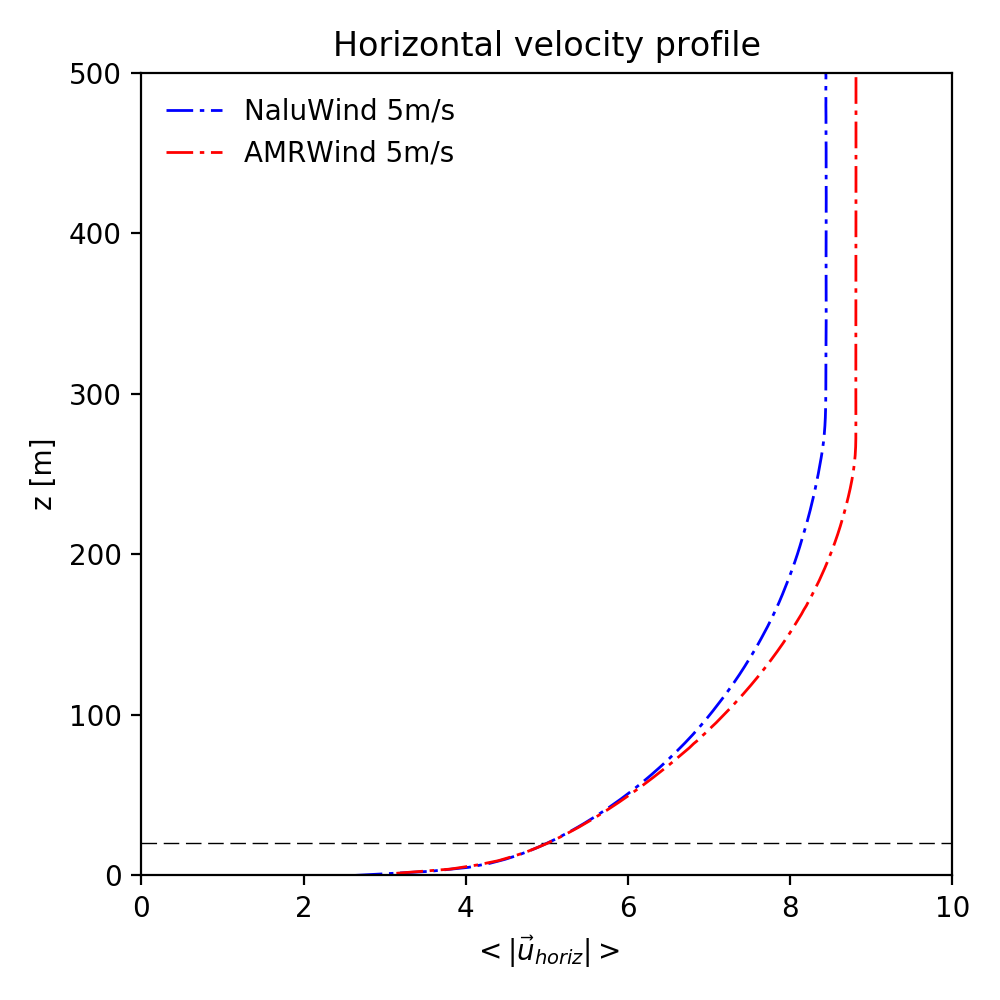
\includegraphics[width=2.5in]{figures/Compare_AMRWind_NaluWind/AMRWind_NaluWind_stable_05ms_mesh2p5_2p5_2p5_WS.png}
  \includegraphics[width=2.5in]{figures/Compare_AMRWind_NaluWind/AMRWind_NaluWind_stable_05ms_mesh2p5_2p5_2p5_Wdir.png}\\
  \caption{\label{fig:CompareAMRvsNaluWind_WSDir} Comparison of
    AMR-Wind and Nalu-Wind velocity profiles.  The dashed horizontal
    line corresponds to the measurement height z=20m. }
\end{figure}
%%%%%%%%%%%%%%%%%%%%%%%%%%%%%%%%%%%%%%%%%%%%%%%%%%%%%%%%%%%%%%%%%%%%

%%%%%%%%%%% Compare Nalu/AMR TI/Temp profiles %%%%%%%%%%%%%%%%%%%%%%
% Postprocessing/ABLStats/AMRWind_NaluWind_stable_05ms_mesh2_5x2_5x2_5_paper.ipynb
\begin{figure} %[hbt!]
  \centering
  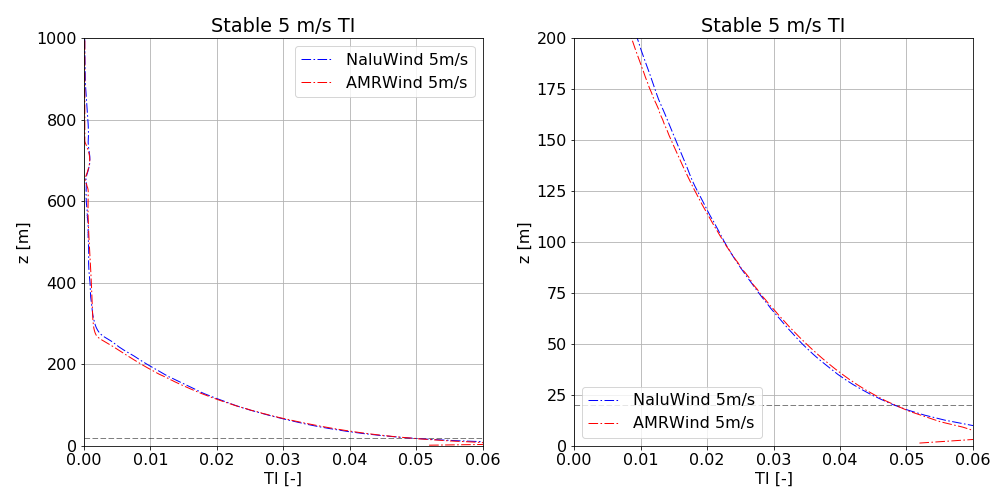
\includegraphics[width=2.5in]{figures/Compare_AMRWind_NaluWind/AMRWind_NaluWind_stable_05ms_mesh2p5_2p5_2p5_TI.png}
  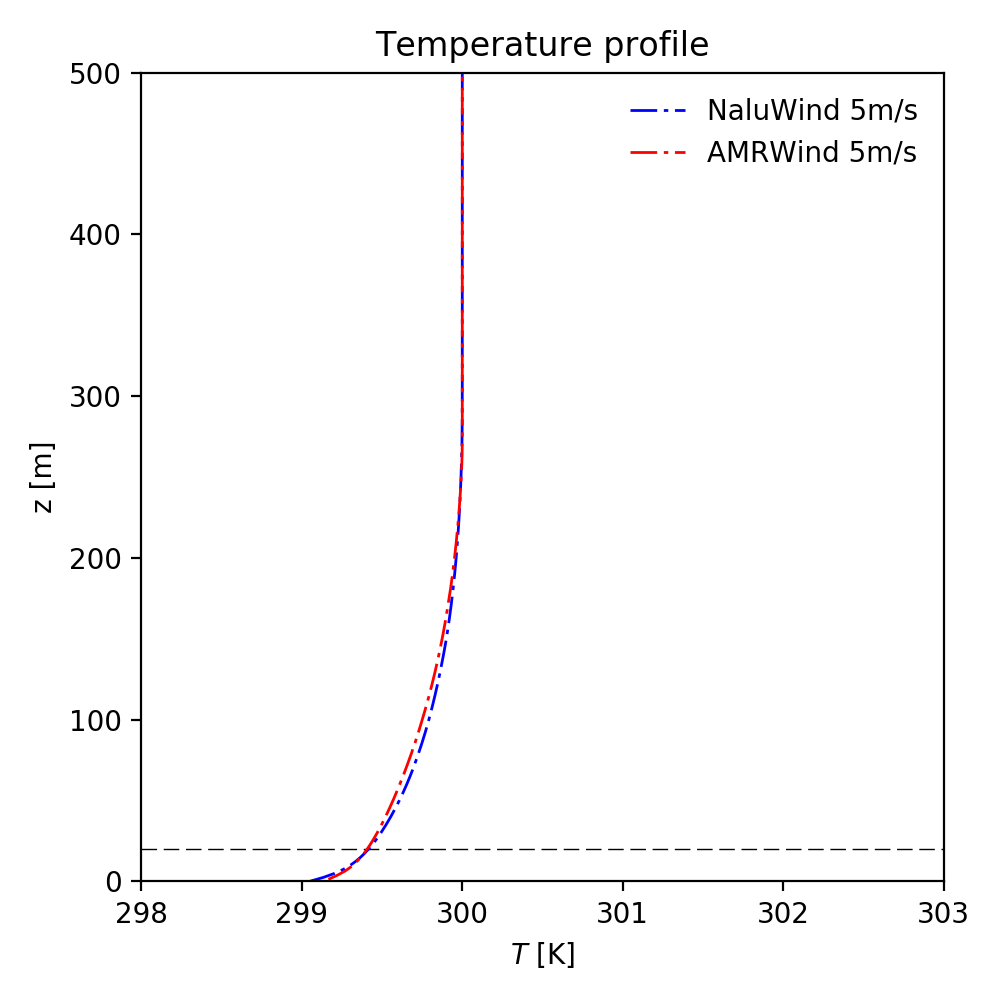
\includegraphics[width=2.5in]{figures/Compare_AMRWind_NaluWind/AMRWind_NaluWind_stable_05ms_mesh2p5_2p5_2p5_T.png}
  \caption{\label{fig:CompareAMRvsNaluWind_TTI} Comparison of AMR-Wind
    and Nalu-Wind turbulence intensity and temperature profiles. The
    dashed horizontal line corresponds to the measurement height
    z=20m.}
\end{figure}
%%%%%%%%%%%%%%%%%%%%%%%%%%%%%%%%%%%%%%%%%%%%%%%%%%%%%%%%%%%%%%%%%%%%

\subsubsection*{Wind spectra and turbulent correlation}

A comparison of the computed wind spectra $S_i(f)$ is shown in figure
\ref{fig:CompareAMRvsNaluSpectra}.

A comparison of the $R_{ij}$ correlation is shown in figure
\ref{fig:CompareAMRvsNaluRij}.

%%%%%%%%%%% Compare Nalu/AMR spectra %%%%%%%%%%%%%%%%%%%%%%%%%%%%%%%%
% Postprocessing/ABLSpectra/AMRWind_NaluWind_Spectra_Stable.ipynb
\begin{figure} %[hbt!]
  \centering
  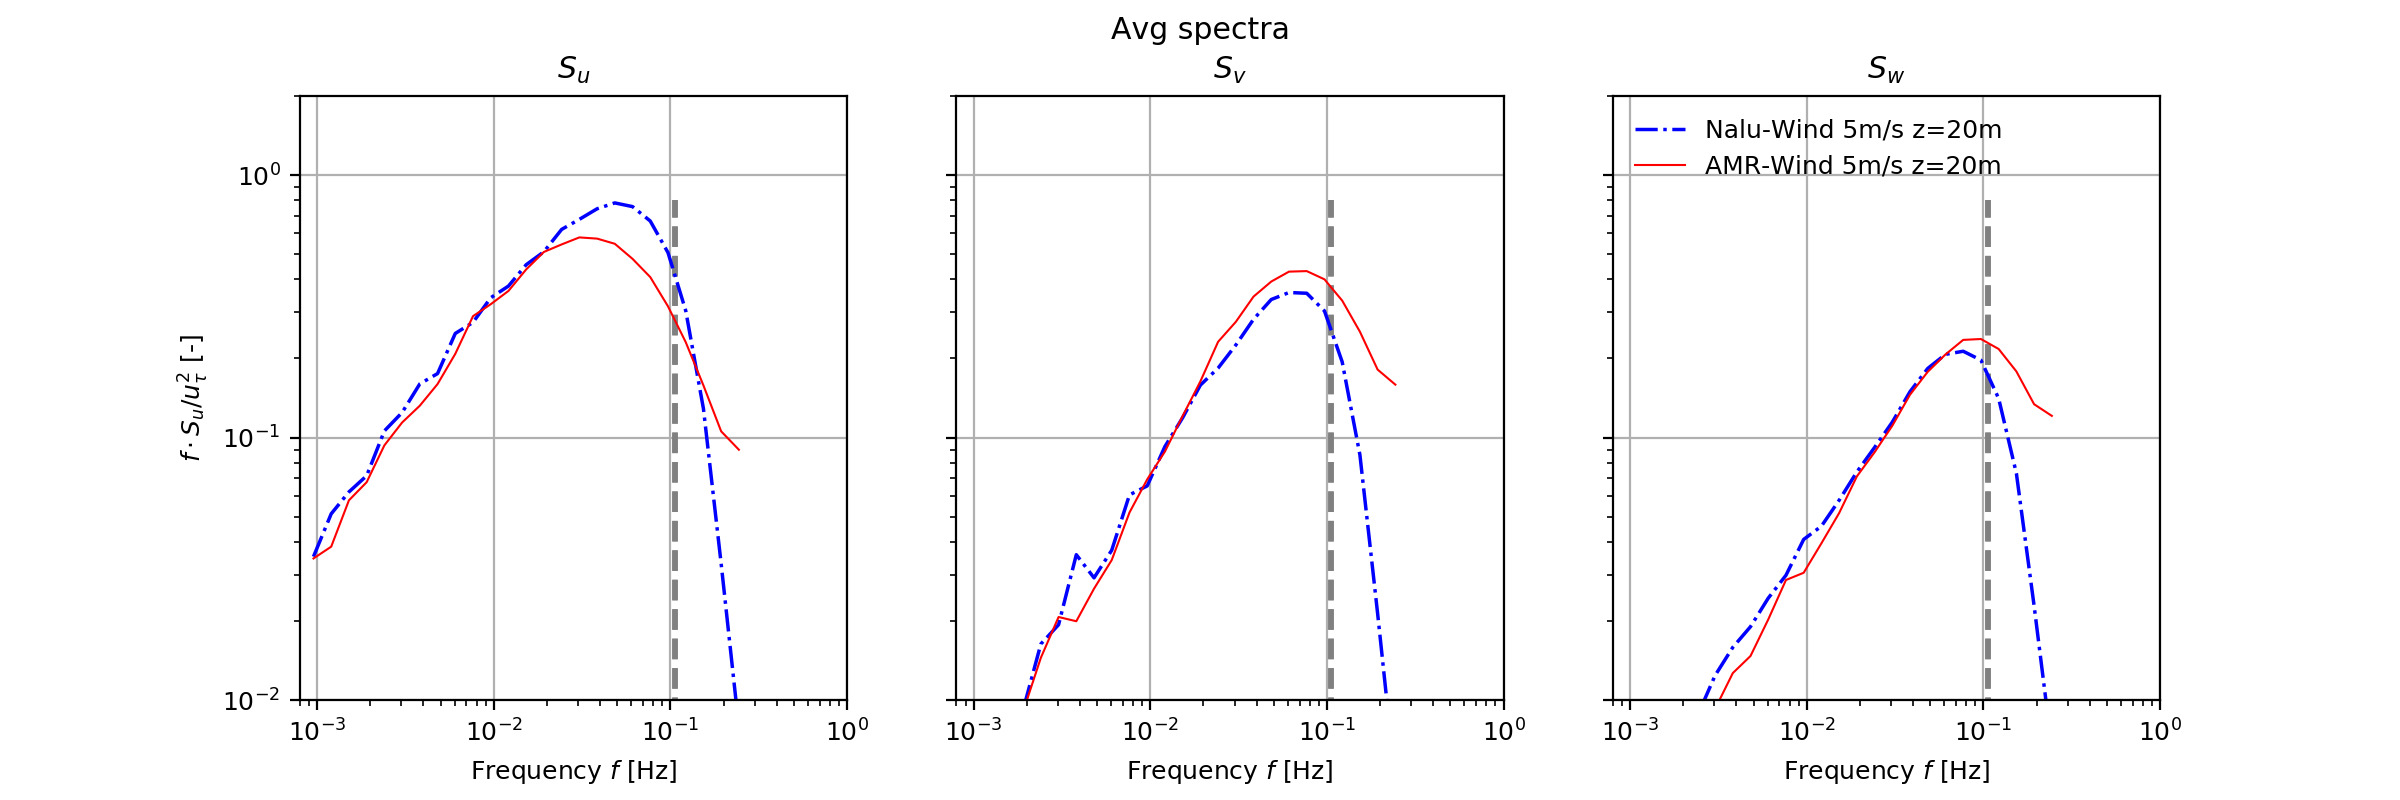
\includegraphics[width=7.0in]{figures/Compare_AMRWind_NaluWind/AMRWind_NaluWind_Spectra_Stable_z20.png}

  \caption{\label{fig:CompareAMRvsNaluSpectra} Comparison of AMR-Wind
    and Nalu-Wind wind spectra at z=20m. }
\end{figure}
%%%%%%%%%%%%%%%%%%%%%%%%%%%%%%%%%%%%%%%%%%%%%%%%%%%%%%%%%%%%%%%%%%%%

%%%%%%%%%%% Compare Nalu/AMR lengthscale %%%%%%%%%%%%%%%%%%%%%%%%%%%%
% Postprocessing/ABLLength/CompareAMRNalu_ABL_Lengthscales.ipynb
\begin{figure} %[hbt!]
  \centering
  \fxnote{UPDATE THIS FIGURE}\\
  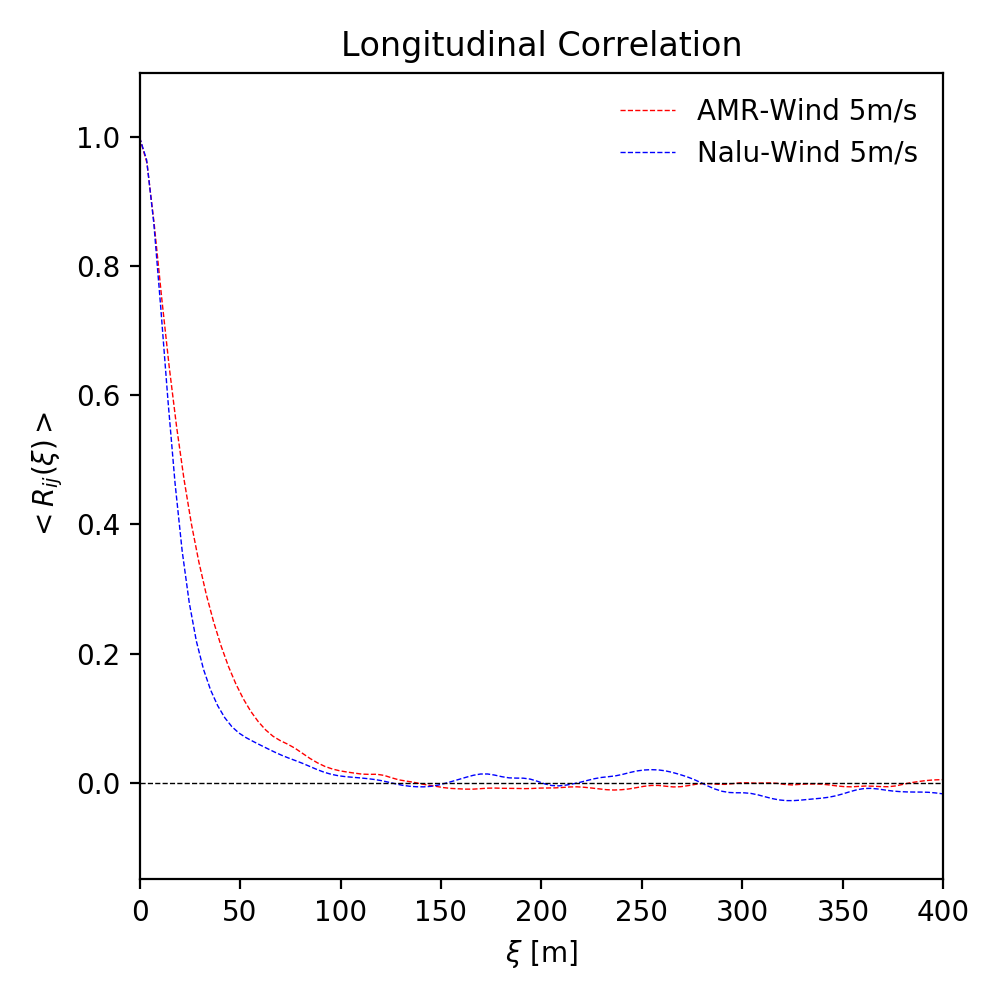
\includegraphics[width=2.5in]{figures/Compare_AMRWind_NaluWind/AMRWind_NaluWind_Lengthscale_Stable_z20_Longitudinal.png}
  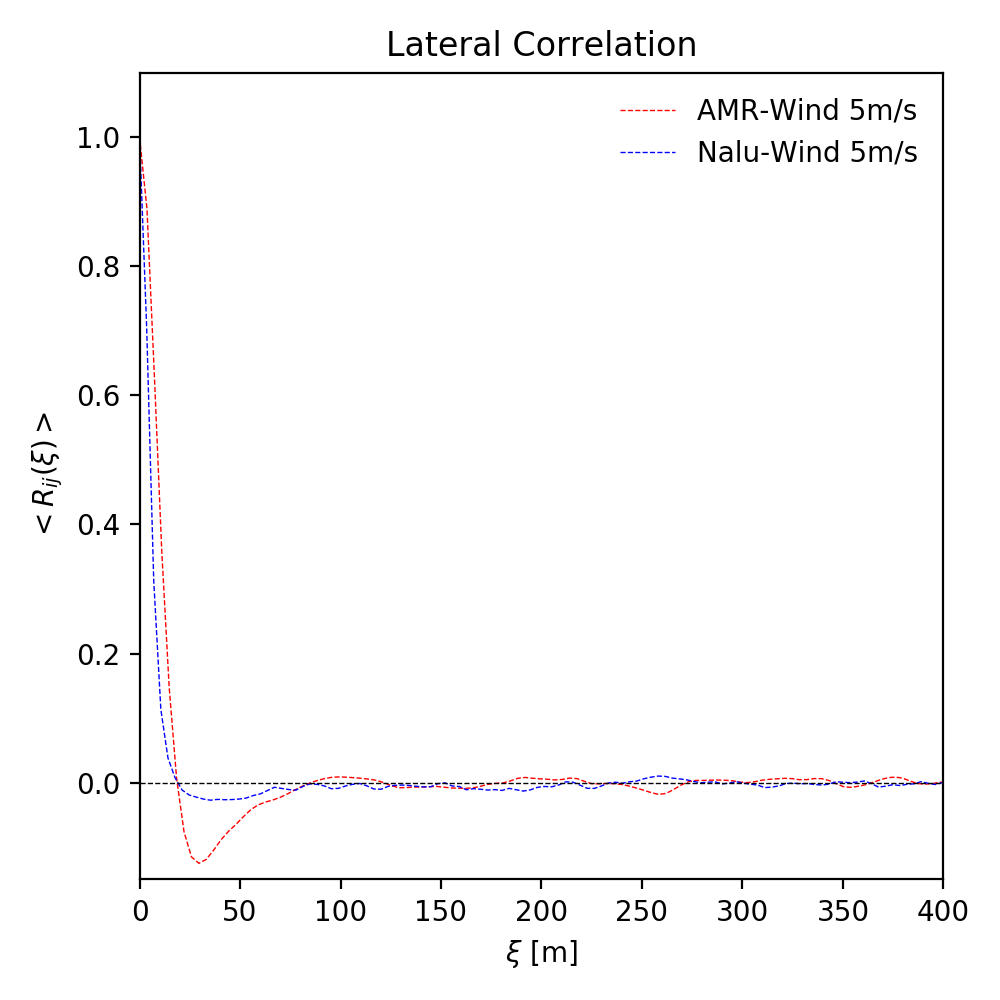
\includegraphics[width=2.5in]{figures/Compare_AMRWind_NaluWind/AMRWind_NaluWind_Lengthscale_Stable_z20_Lateral.png}

  \caption{\label{fig:CompareAMRvsNaluRij}
    Comparison of AMR-Wind and Nalu-Wind $\langle R_{ij}
    \rangle$ correlation at z=20m. }
\end{figure}
%%%%%%%%%%%%%%%%%%%%%%%%%%%%%%%%%%%%%%%%%%%%%%%%%%%%%%%%%%%%%%%%%%%%

\subsubsection*{Computational efficiency}
How much faster is AMR-Wind compared to Nalu-Wind?  \\
\fxnote{PUT SOME NUMBERS HERE FROM MIKE}

\subsection{Comparison of stable offshore ABL for different wind speeds and stabilities}

\subsubsection{ABL integrated quantities}
Describe integrated quantities

\subsubsection{Horizontally averaged profiles}

\subsubsection{Wind spectra and turbulence statistics}

The Kaimal model for spectra \cite{kaimal1973turbulence,
  cheynet2017spectral} for neutral atmospheric conditions:
\begin{equation}
  \label{eq:kaimal}
  \frac{fS_i}{u_\tau^2} = \frac{a_i(fz/\bar{U})}{\left(1+b_i(fz/\bar{U})^{\alpha_i}\right)^{\beta_i}}
\end{equation}

%%%%%%%%%%%%%%% KAIMAL MODEL PARAMETERS %%%%%%%%%%%%%%%%%%%%%%%%%%%%%%%%%%%
\begin{table}[h]
\caption{\label{tab:KaimalParameters} Parameters for Kaimal model}
\centering
\begin{tabular}{ccccc}
  \hline
  Index $i$& $a_i$ & $b_i$ & $\alpha_i$  & $\beta_i$ \\
  \hline
  $u$      & 105.0 & 33.0  & 1           & 5/3  \\
  $v$      &  17.0 &  9.5  & 1           & 5/3  \\
  $w$      &   2.1 &  5.3  & 5/3         &   1  \\
\hline
\end{tabular}
\end{table}


%%%%%%%%%%% Grid resolution spectra figure %%%%%%%%%%%%%%%%%%%%%%%%%
% Created in Postprocessing/ABLSpectra/Stable_Spectra_Allz.ipynb
\begin{figure}[hbt!]
  \label{fig:ABLSpectra_AllZ}
  \centering
  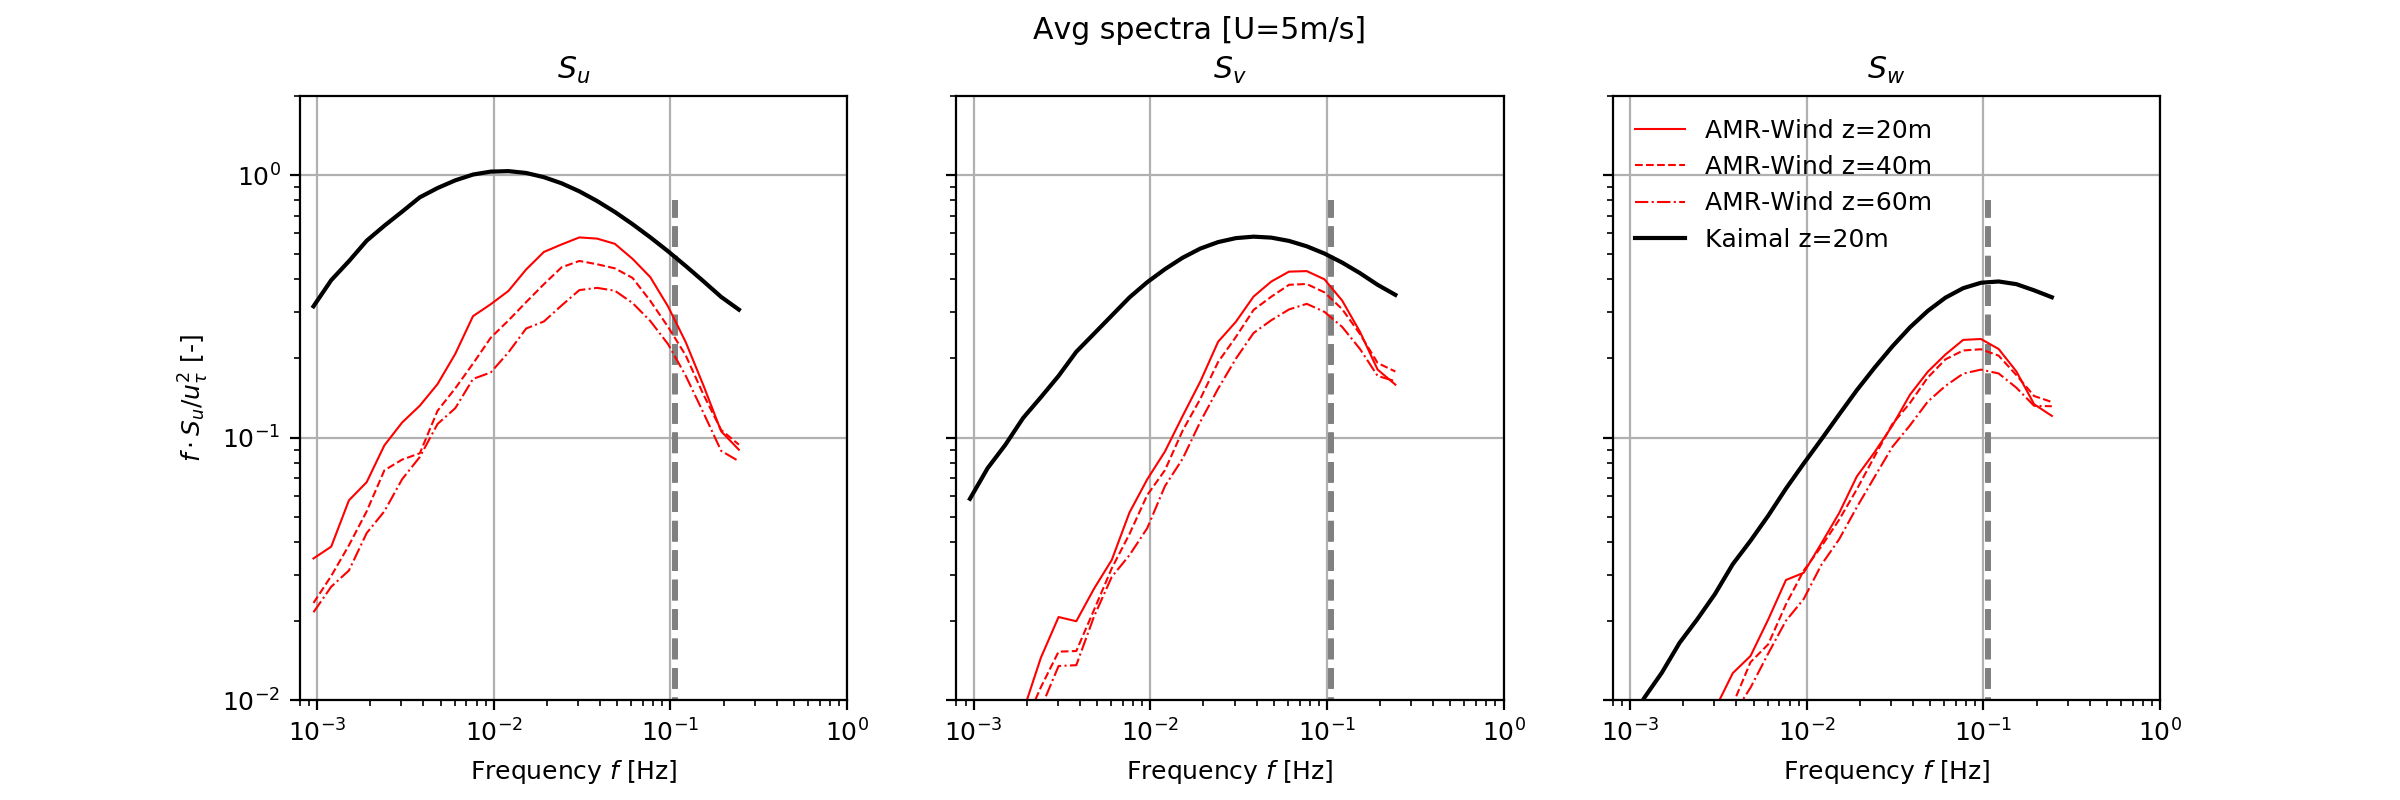
\includegraphics[width=7.0in]{figures/Stable_Spectra_AllZ_05ms.png}\\
  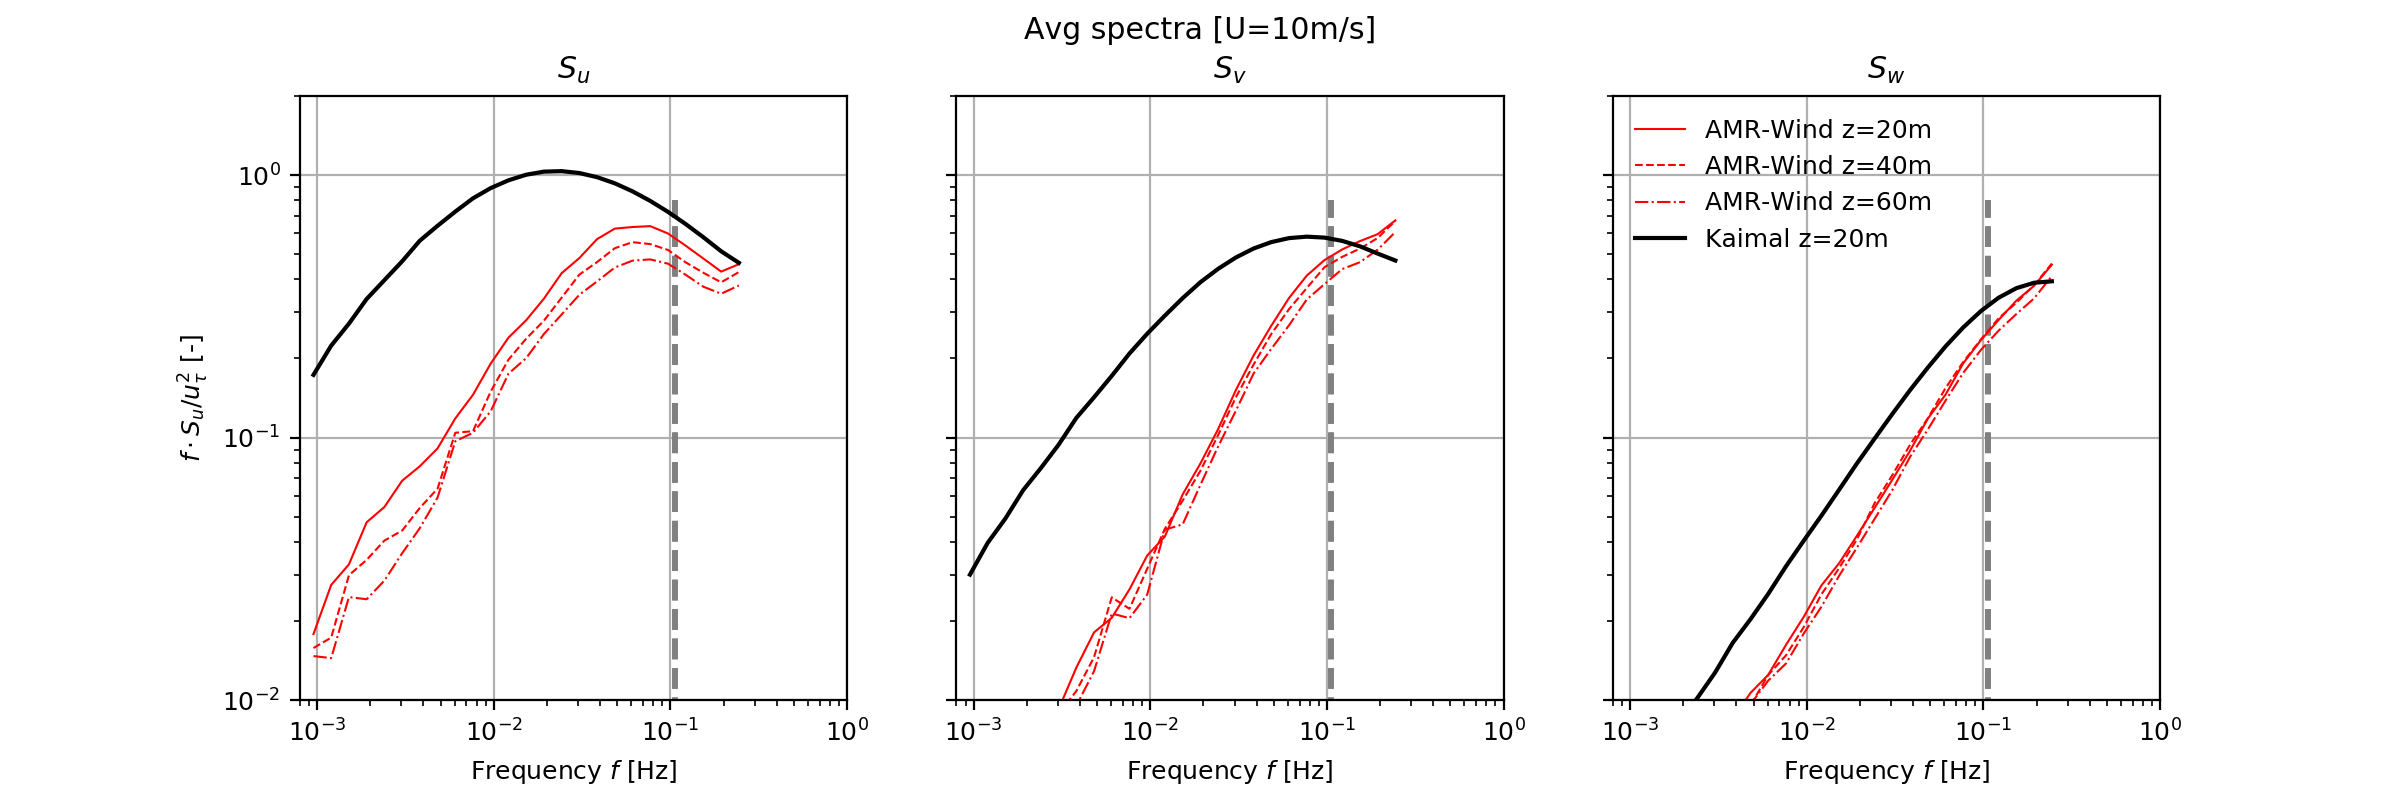
\includegraphics[width=7.0in]{figures/Stable_Spectra_AllZ_10ms.png}\\
  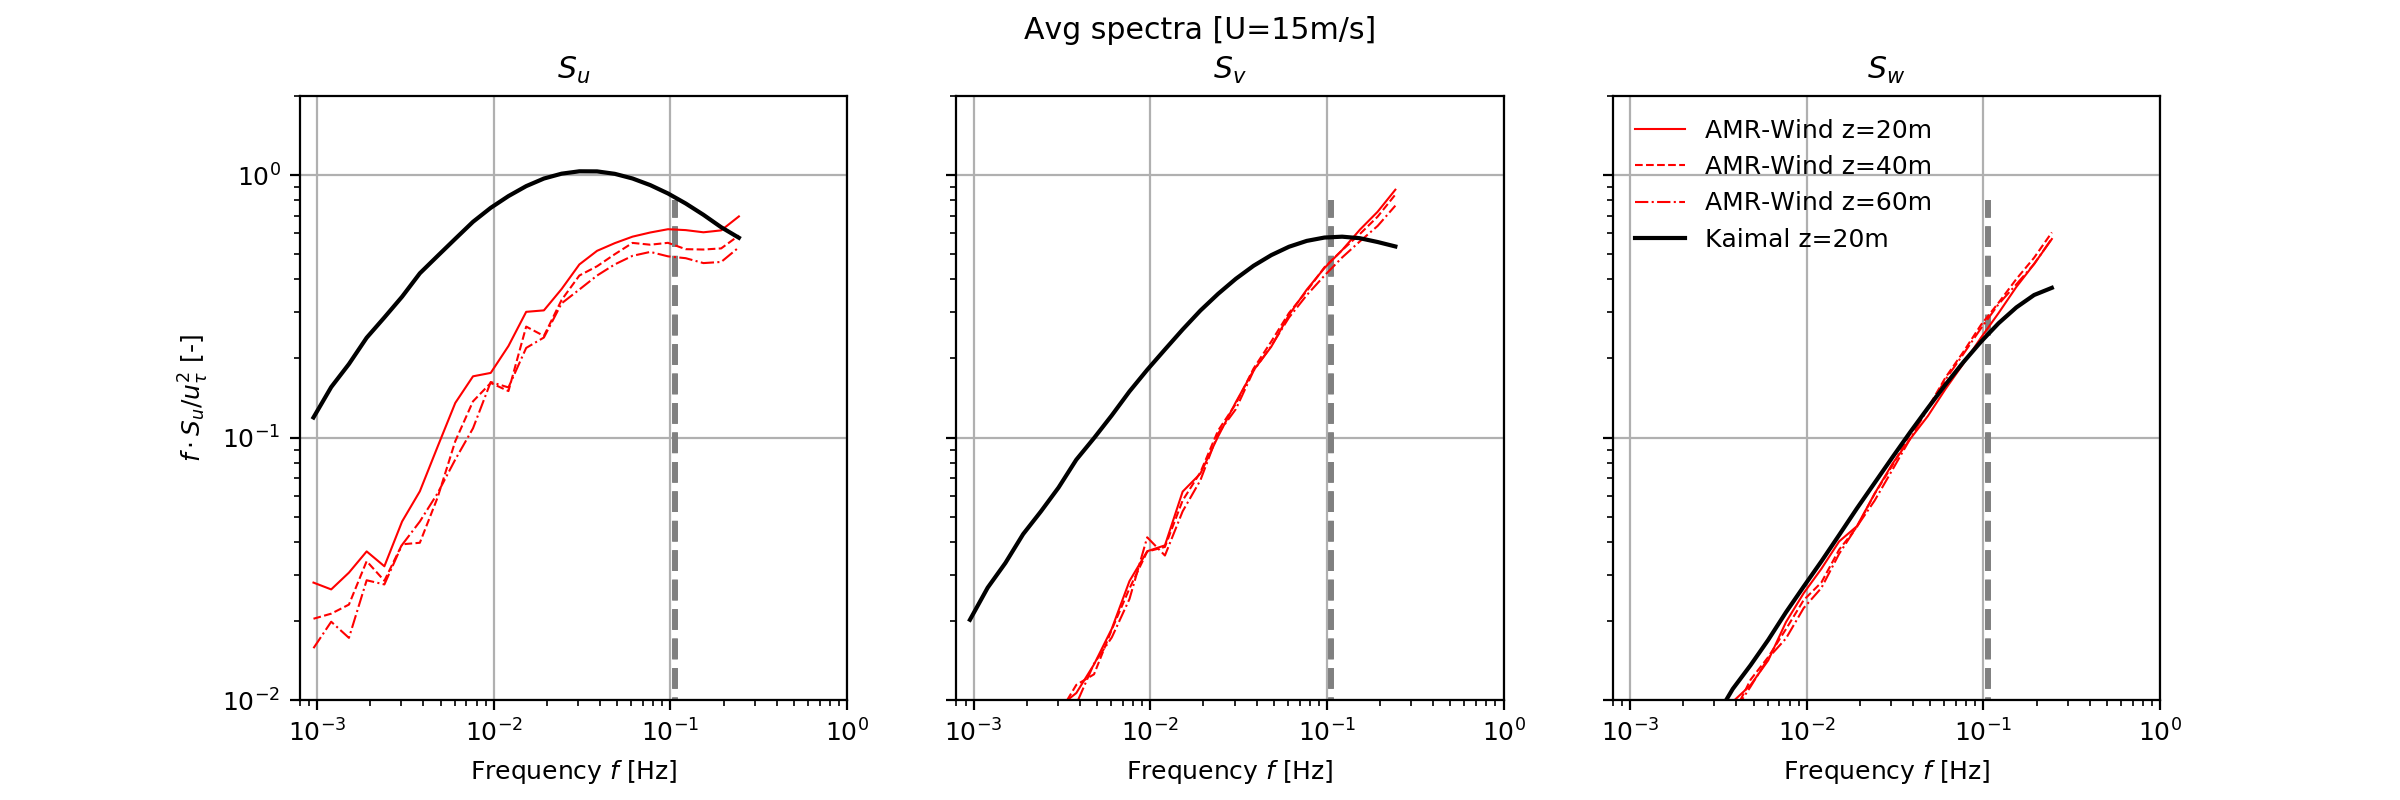
\includegraphics[width=7.0in]{figures/Stable_Spectra_AllZ_15ms.png}
  \caption{Calculation of the wind spectra $S_i$ for LES of stable
    5m/s, 10m/s, and 15m/s cases at z=20m, 40m, and 60m.  The black
    vertical lines correspond to the maximum resolvable frequency
    $f_{max}$ according to equation (\ref{eq:fmax}). }
\end{figure}
%%%%%%%%%%%%%%%%%%%%%%%%%%%%%%%%%%%%%%%%%%%%%%%%%%%%%%%%%%%%%%%%%%%%


\subsubsection{Comparison with neutral and unstable conditions}


%%%%%%%%%%% All stability correlation figure %%%%%%%%%%%%%%%%%%%%
% created in Postprocessing/ABLLength/CompareAll_ABL_Lengthscales.ipynb 
\begin{figure}[hbt!]
  \label{fig:AllStabilityRij}
  \centering
  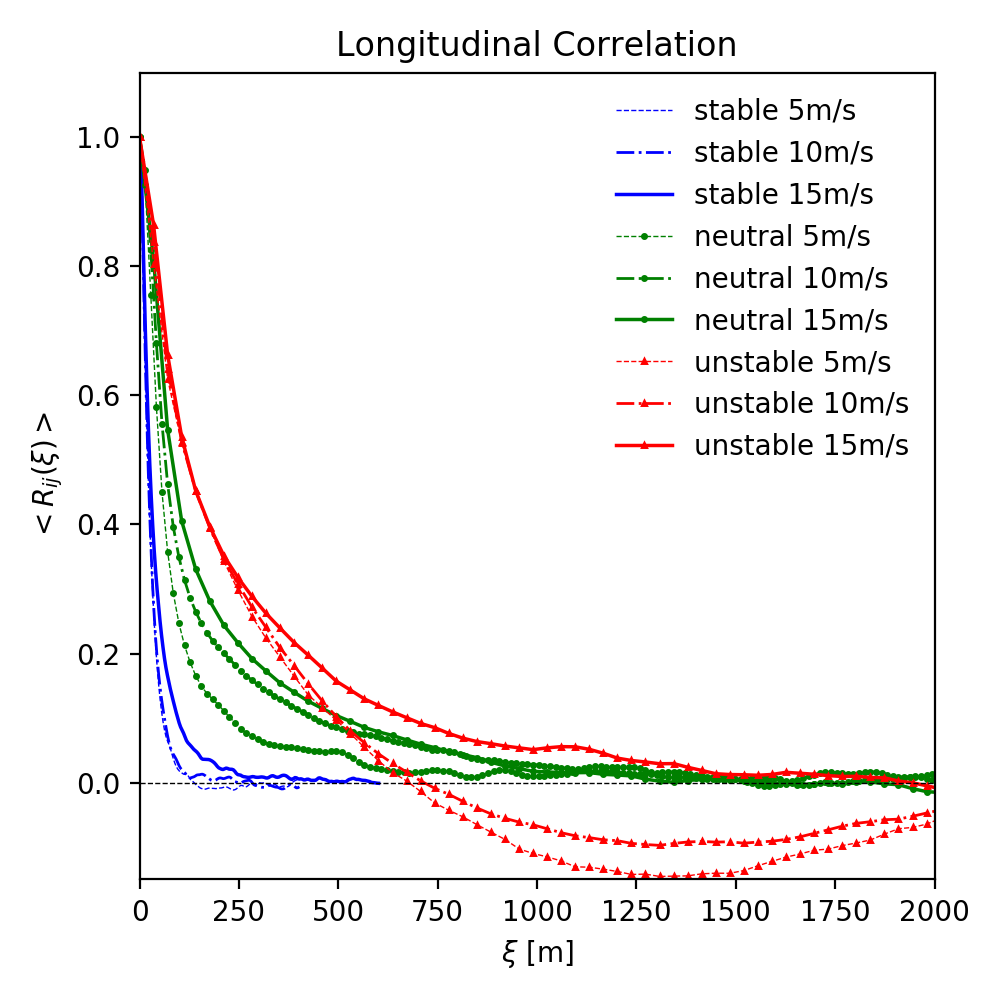
\includegraphics[width=3in]{figures/AllStability_Rij_Longitudinal.png}
  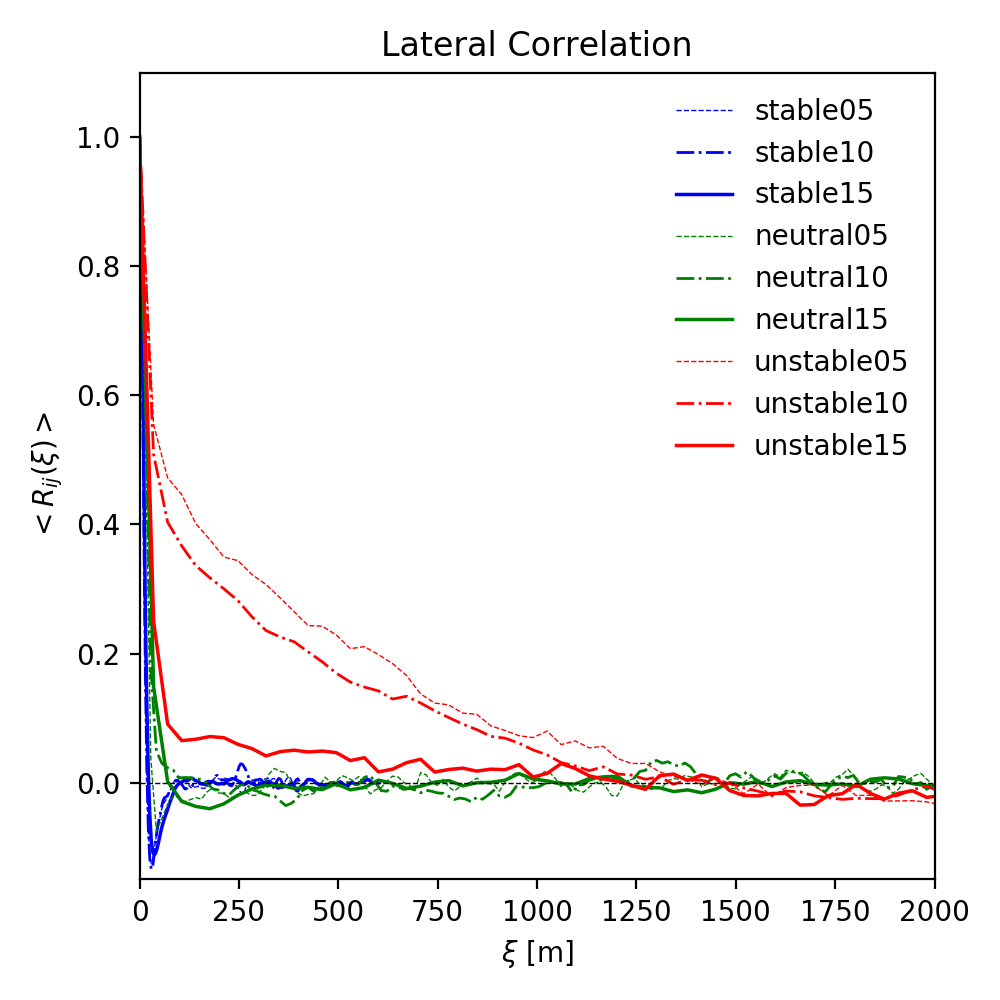
\includegraphics[width=3in]{figures/AllStability_Rij_Lateral.png}
  \caption{Calculation of the averaged longitudinal and lateral
    $R_{ij}(\xi)$ coefficient at $z$=20m for all ABL stability cases.}
\end{figure}
%%%%%%%%%%%%%%%%%%%%%%%%%%%%%%%%%%%%%%%%%%%%%%%%%%%%%%%%%%%%%%%%%%%%

%%%%%%%%%%%%%%% GRID STUDY: INTEGRAL LENGTH %%%%%%%%%%%%%%%%%%%%%%%%%%%%%%%%%%%
\begin{table}
\caption{\label{tab:StabilityStudyLscale} The calculated turbulent
  integral lengthscale for each of atmospheric stabilities} \centering
\begin{tabular}{ccccc}
  \hline
  Stability   & Wind speed & Longitudinal L [m] & Lateral L [m] \\
  \hline
  Stable      &   5 m/s  & 0.0           & 0.0        \\
  Stable      &  10 m/s  & 0.0           & 0.0        \\
  Stable      &  15 m/s  & 0.0           & 0.0        \\
  Neutral     &   5 m/s  & 110.435741    & 15.245327  \\
  Neutral     &  10 m/s  & 165.398368    & 20.634052  \\
  Neutral     &  15 m/s  & 184.081967    & 22.961169  \\
  Unstable    &   5 m/s  & 187.868710    & 270.538753 \\
  Unstable    &  10 m/s  & 177.457502    & 215.027457 \\
  Unstable    &  15 m/s  & 263.475309    & 67.999898  \\
\hline
\end{tabular}
\end{table}
%%%%%%%%%%%%%%%%%%%%%%%%%%%%%%%%%%%%%%%%%%%%%%%%%%%%%%%%%%%%%%%%%%%%
